%!TEX root = ../../../super_main.tex
\section{Improved Design of the \emph{Category Tool}}
\label{sec:improved_design}

\todo{Hvis der blvier bygget et appendix til markup så henvis til det.}
We decided to make a major rework of the current design of the \ct. The new design must be an improvement to the old design, and should not suffer from the same design flaws. Furthermore, the new design should improve usability and should ideally never crash when used. \todo[inline]{TODO START NIKLAS FIXERTING - skriv at vi har fjerner funktionalitet} Besides this, the tool should not implement any unwanted features, such as colored categories or sub categories.
\todo[inline]{TODO START NIKLAS FIXERTING}
\\\\
Instead of just implementing an incremental design straight ahead, some initial markup of the design, which has gone through some iterations, has been made. This markup is then later used in the implementation of the design. Different parts of this markup are described throughout this section.

\subsection{Separation of Categories by Type}
The customers have previously described that they would like to be able to copy categories between citizens. To accommodate this, it was decided that categories must be ``bound'' to an institution instead of actual citizens. This will ensure that the categories for a specific institution are independent of any citizen. When a category is assigned to a citizen, the content (pictograms) should be copied to a new category (with the same name) which then belongs to the citizen. This will allow guardians to make changes to a specific citizen-assigned category without affecting other categories. 
\\\\
Take for instance an institution that have the category \emph{Toys} which has some pictograms associated with it. The guardians of this institution then decide that citizens \emph{A} and \emph{B} should have access to use this category, therefore they copy the \emph{Toys} category to both citizens. However, \emph{A} is unsatisfied with the new category and feels that it is missing his favorite toy. To make \emph{A} happy, the guardians then add a pictogram of his toy to \emph{A}'s category. Because of the way the system is designed, this action should have no effect on the the \emph{Toys} category of \emph{B}.
\\\\
This idea of separating categories into institution and citizen-assigned categories can be difficult to understand for new users, so it will require the user-interface to be clear about which categories are being viewed or modified. Therefore, when using the \ct the user should always be aware of what type of categories are being presented.
\\\\
Clarification as to where the user currently is in the \ct should be indicated by use of the \androidinline{ActionBar} mentioned in \secref{sec:giraf_activity_actionbar}. This bar should clearly state whose categories are shown at the moment.

\subsection{Home Screen}
\label{sec:home_screen}
When opening the \ct, the user should be presented with a screen similar to the markup seen in \figref{fig:improved_design_launch_screen}. As seen in the figure, the user is presented with a list (to the left). This list contains all of the categories that are bound to the specific institution, based on the affiliation of the currently logged in guardian. On the right side of the screen, the user is presented with a small introduction to the tool. For instance, the arrow-text reads \translated{Vælg en kategori for at se dens indhold}{Choose a category to see its content}. This will help to user to understand that the left-side contains categories, and that they are clickable. On the right, the user is also presented with two buttons, namely \translated{Opret ny kategori}{Create new category} and \translated{Administrer borgere}{Administrate citizens}.

\begin{figure}[!htbp]
    \centering
    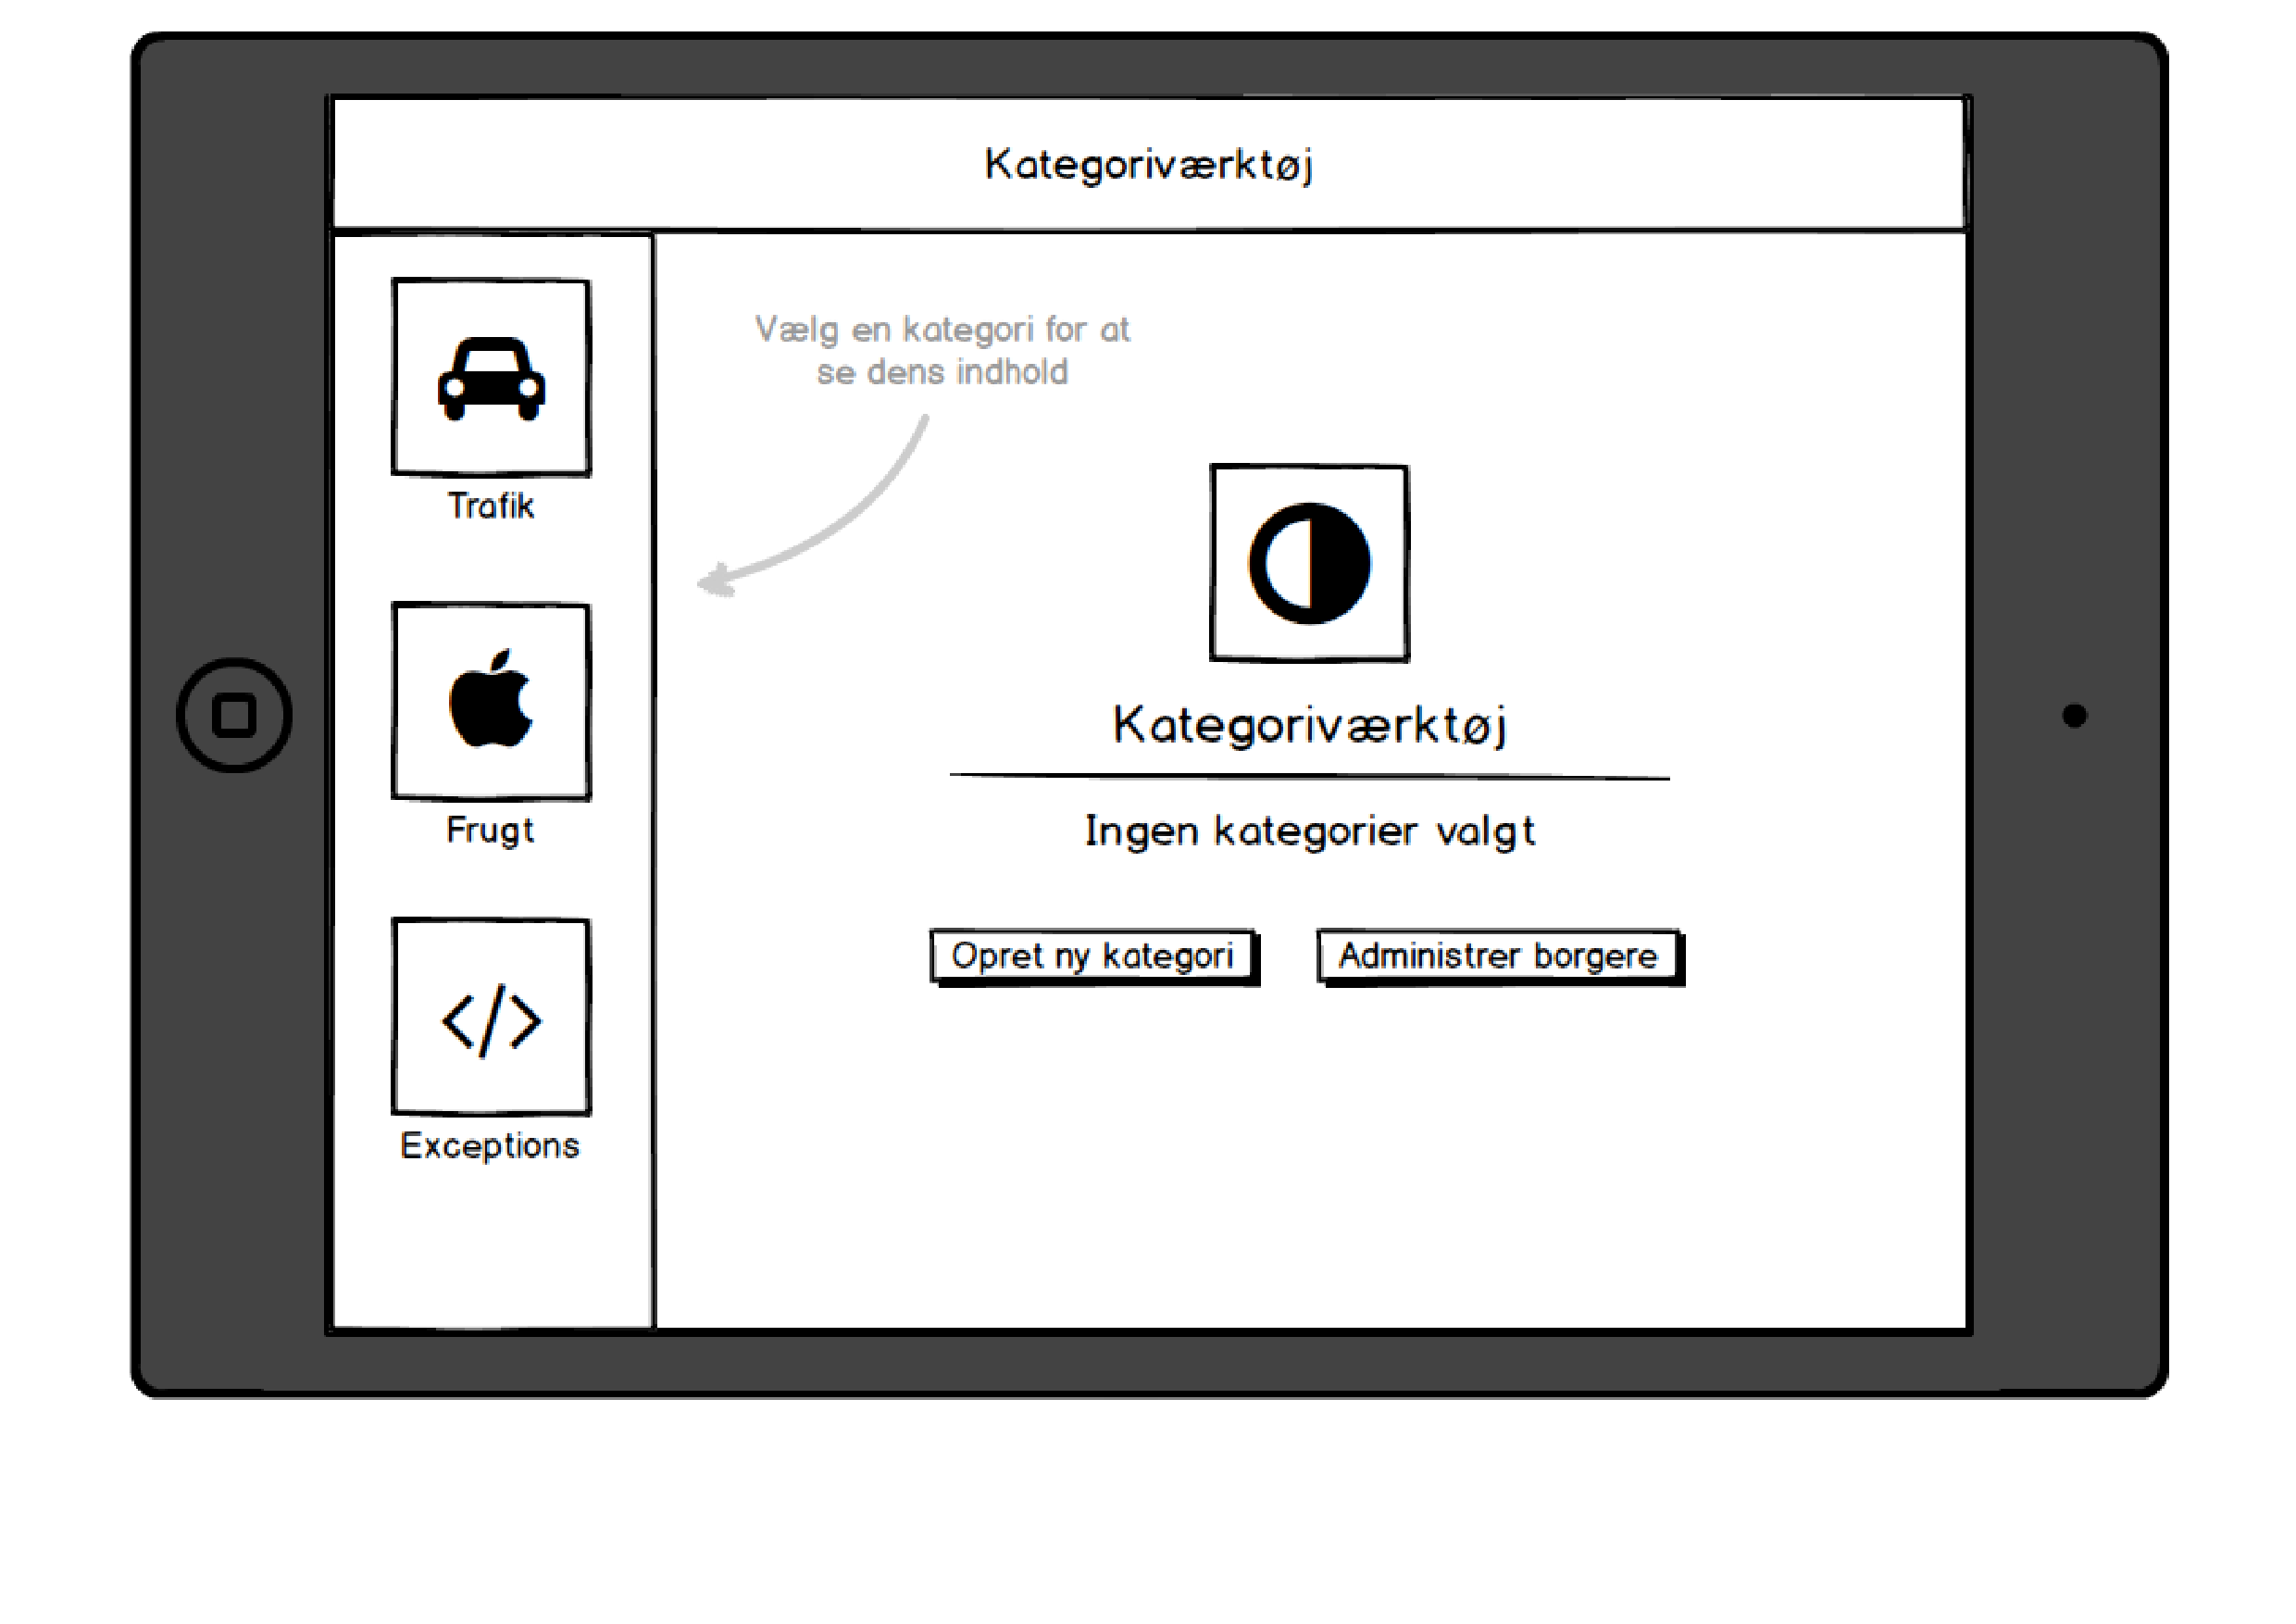
\includegraphics[width=0.75\textwidth]{sprint_two/improved_design/launch_screen}
    \caption{Markup of the home screen}
    \label{fig:improved_design_launch_screen}
\end{figure}

\FloatBarrier

\subsection{Category Selected Screen}
\label{sec:category_selected_screen}
Whenever the user selects a category (in the menu on the left), a screen similar to either \figref{fig:improved_design_category_selected_1} or \figref{fig:improved_design_category_selected_2} should be shown, depending on the presence of pictograms in the category.\\

If the category contains no pictograms, a guide will be shown which will inform the user on how to add pictograms and how to copy the category to citizens. This will inform users on what the different buttons do. However, if the user is new to the system and needs to work on already existing categories, these buttons could possibly be a bit confusing. \\

\begin{figure}[!htbp]
    \centering
    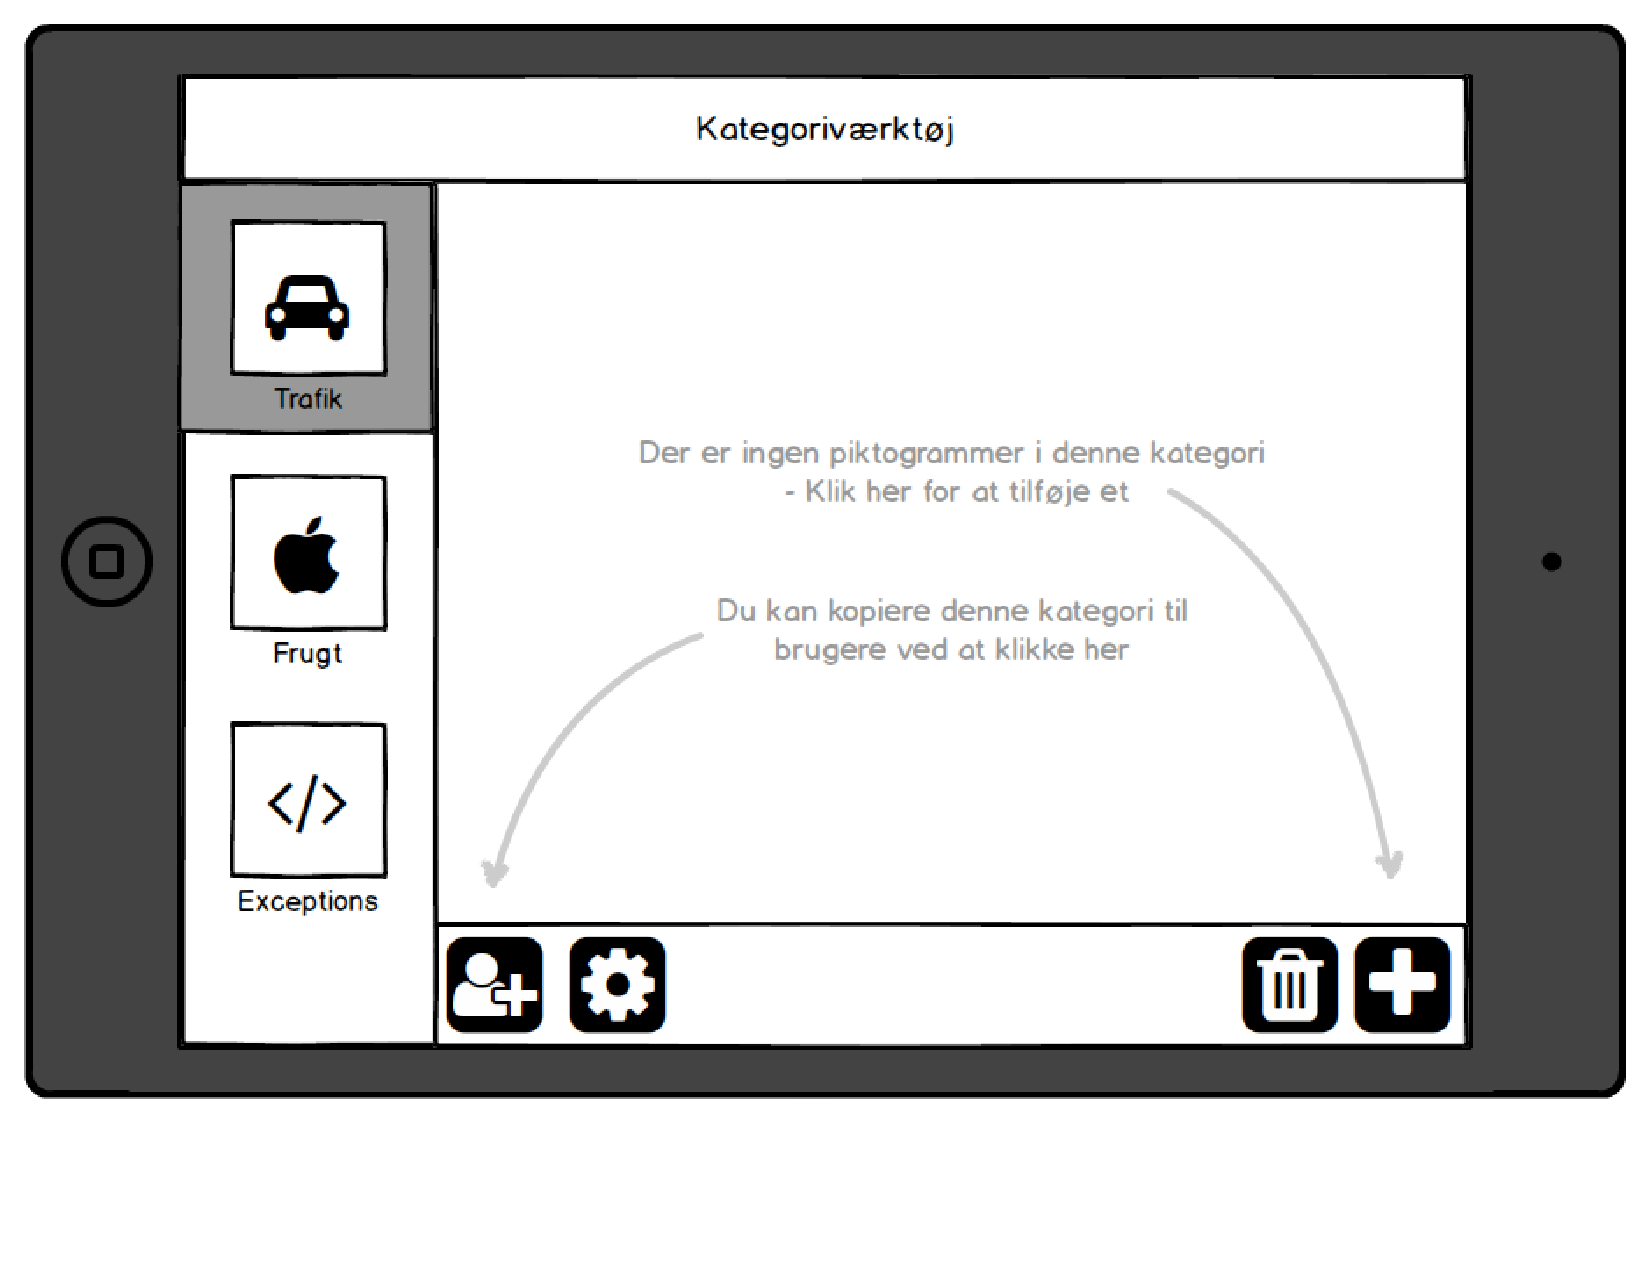
\includegraphics[width=0.75\textwidth]{sprint_two/improved_design/category_selected_1}
    \caption{Markup of the category selected screen without pictograms}
    \label{fig:improved_design_category_selected_1}
\end{figure}

\FloatBarrier

The user will be presented with a screen similar to \figref{fig:improved_design_category_selected_2} if the currently selected category contains pictograms. This screen will present the user with a grid of pictograms in the selected category. The user will be able to scroll through the grid if there are more pictograms than available screen estate. 

\begin{figure}[!htbp]
    \centering
    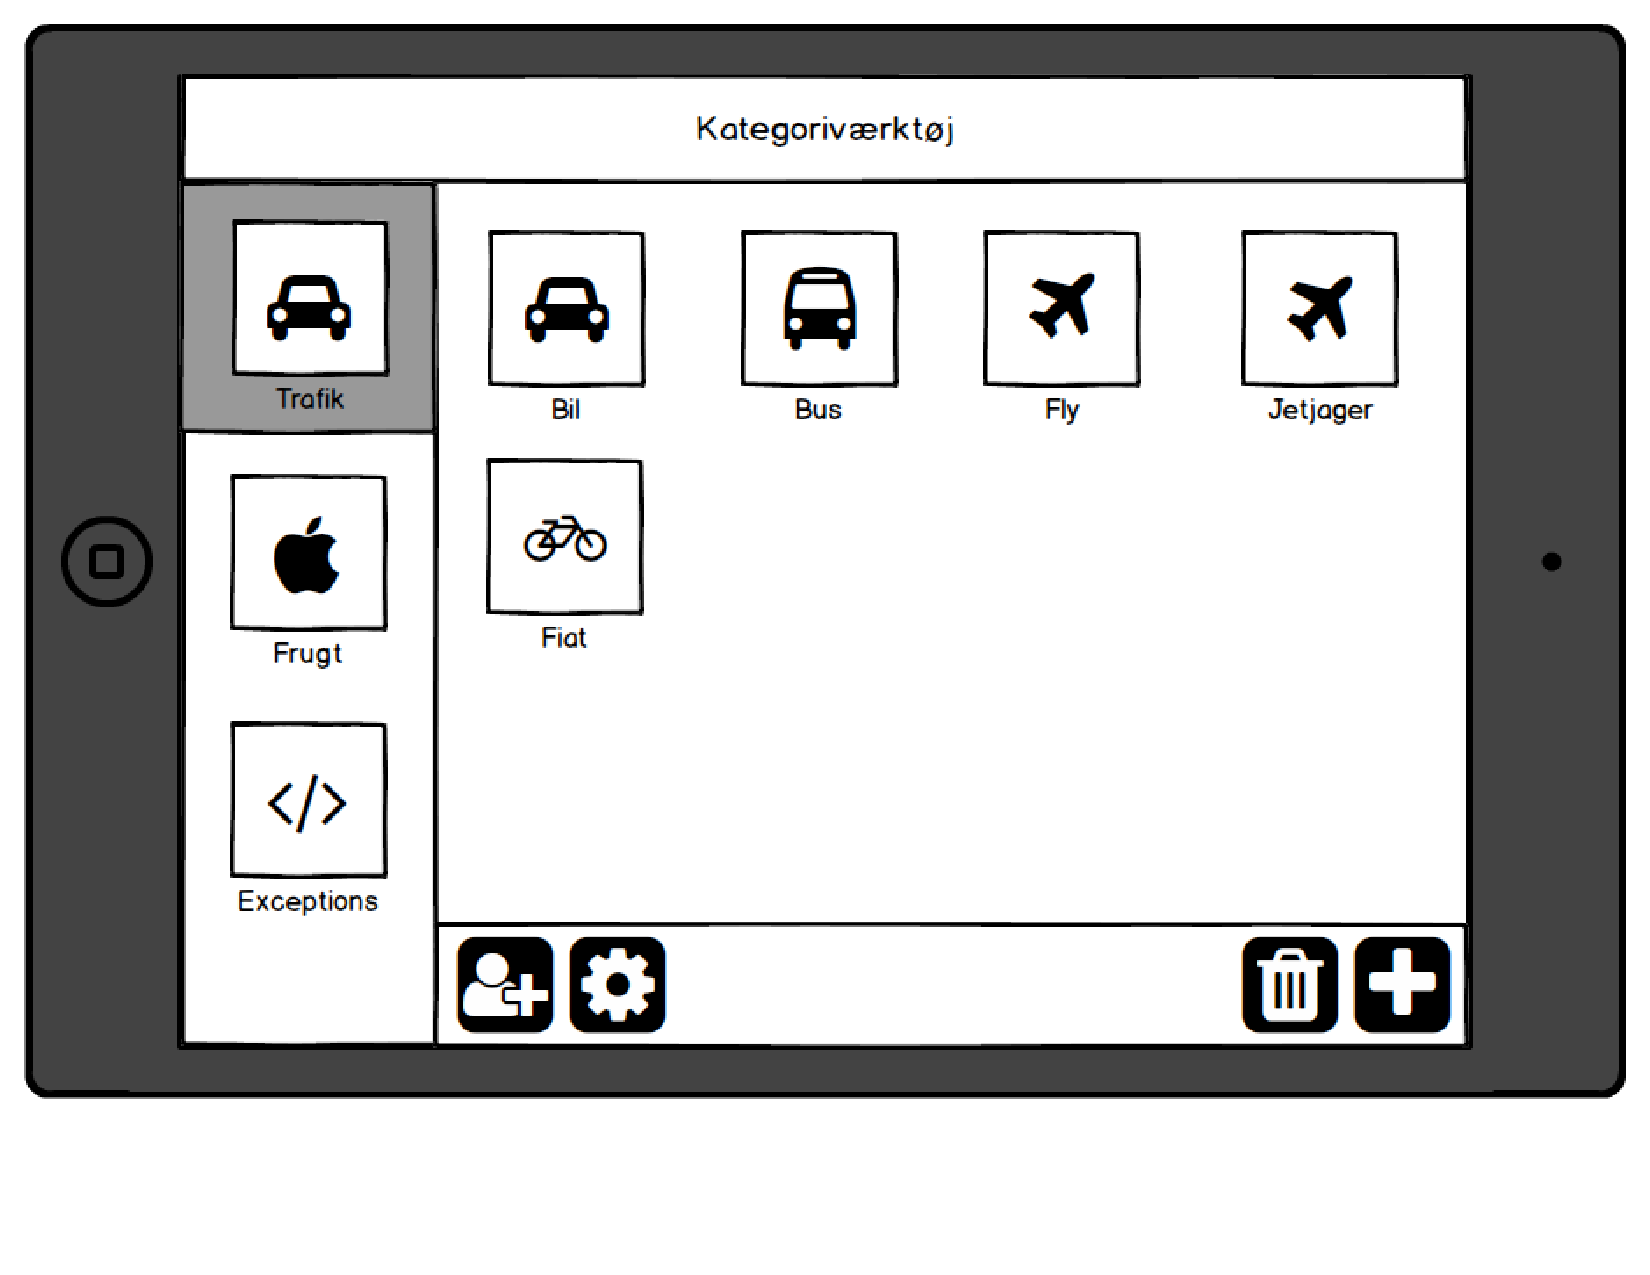
\includegraphics[width=0.75\textwidth]{sprint_two/improved_design/category_selected_2}
    \caption{Markup of the category selected screen with pictograms}
    \label{fig:improved_design_category_selected_2}
\end{figure}

\FloatBarrier

\subsection{Creation and Modification of Categories}
To accommodate the need for creating and removing categories, the following screens have been designed. The category creation screen seen on \figref{fig:improved_design_create_category} will be displayed whenever the \translated{Opret ny kategori}{Create new category} button is pressed on the home screen (see \figref{fig:improved_design_launch_screen}). The point of this screen is to guide the user in the creation of a new category. There are two points to consider when creating a category, namely choosing the eloquent pictogram and title representing the category. To make this clear to the user, two helping arrows have been added, which read \translated{Vælg et piktogram}{Choose a pictogram} and \translated{Skriv en titel}{Write a title}. These arrows have been added so that the user knows that the pictogram-box is clickable and so that it is clear that you are able to write text in the text-box. 

\begin{figure}[!htbp]
    \centering
    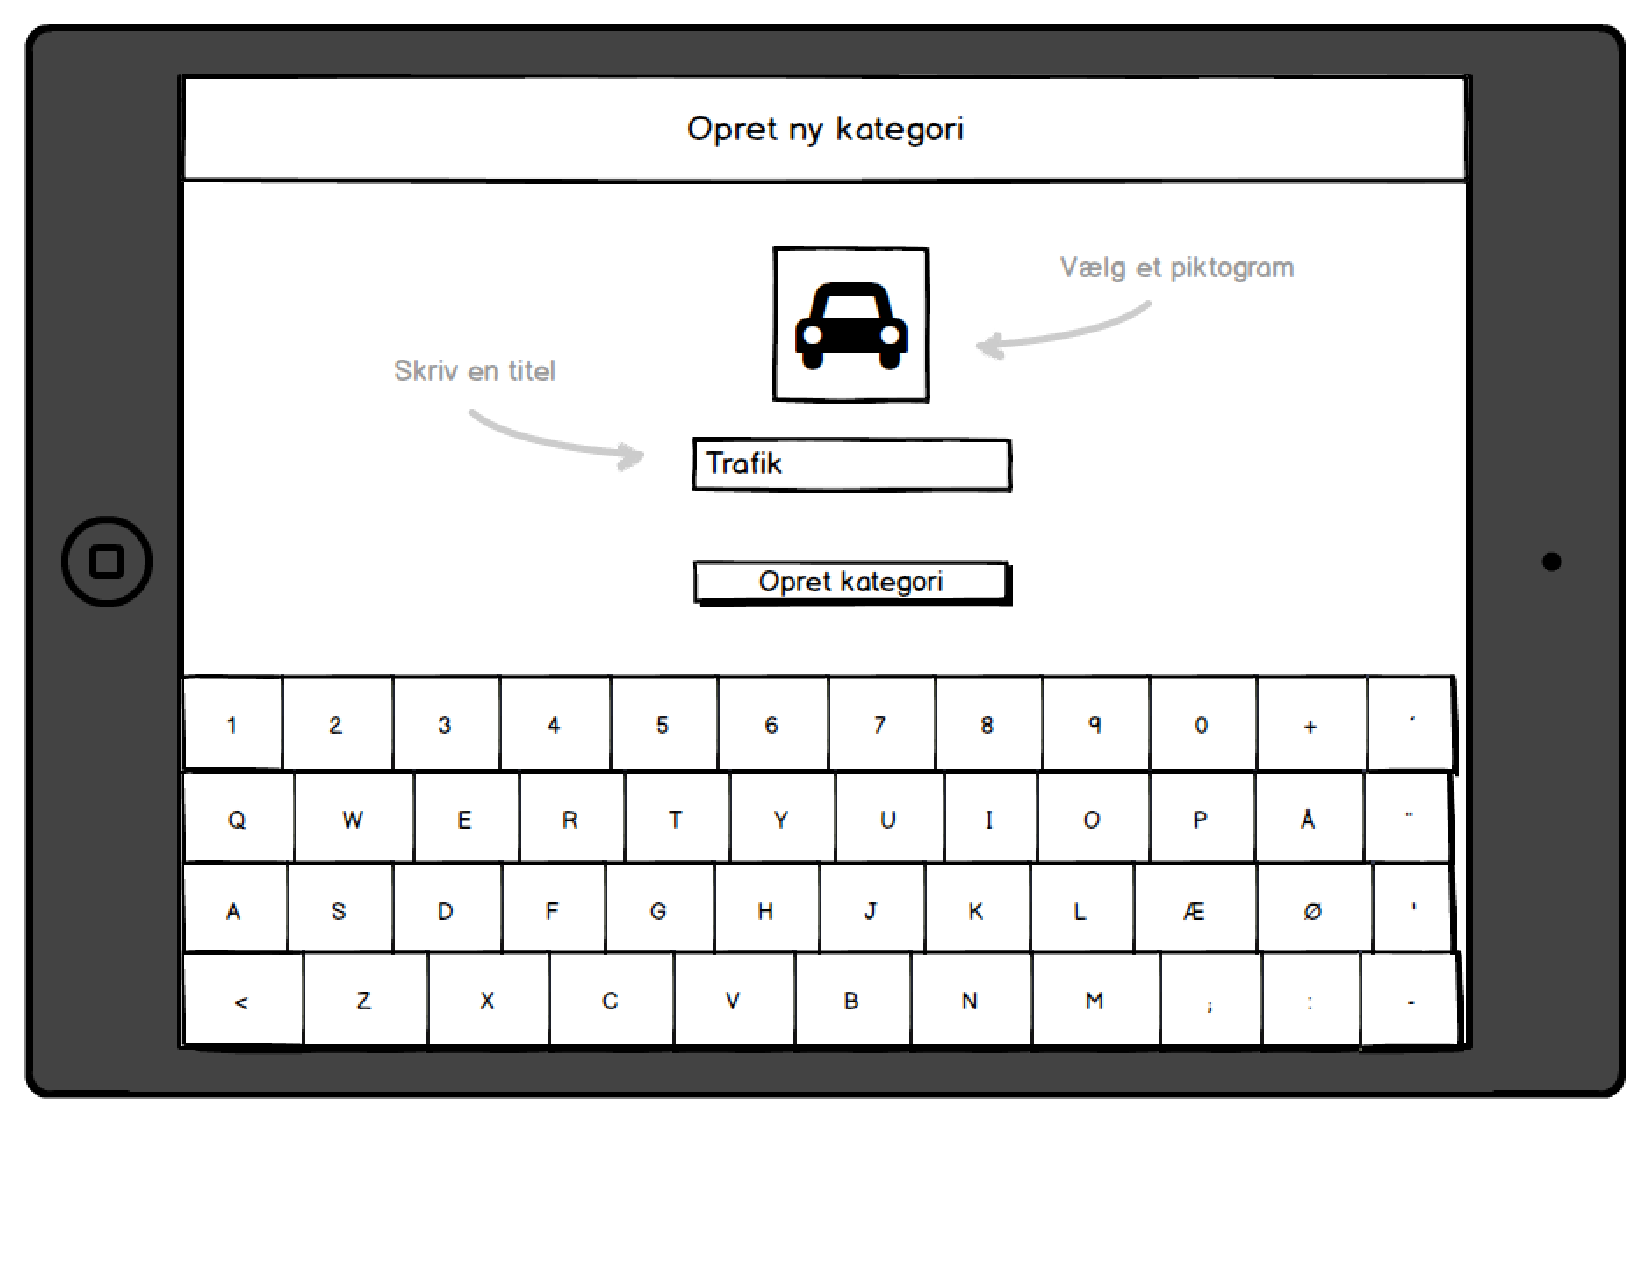
\includegraphics[width=0.75\textwidth]{sprint_two/improved_design/create_category}
    \caption{Markup of the category creation screen}
    \label{fig:improved_design_create_category}
\end{figure}

\FloatBarrier

A user might want to change something regarding a category or deleting a category altogether. To do this, the user must first select a category, then press the cogwheel on the bottom (see \figref{fig:improved_design_category_selected_2}). This will open the dialog-box shown in \figref{fig:improved_design_category_settings}. Here, the user is presented with two buttons, namely \translated{Slet kategori}{Delete category} and \translated{Gem ændringer}{Save changes}. Furthermore, the user is presented with the helpful text \translated{Her kan du ændre piktogrammet og titlen for kategorien}{Here you can change the pictogram and the title for the category}. This dialog does not contain any helpful arrows, because it was deemed unnecessary at this point since the user should be familiar with the way categories are structured. One thing that can be problematic with this design is, that some users might find it hard to figure out how to get this dialog opened. 

\begin{figure}[!htbp]
    \centering
    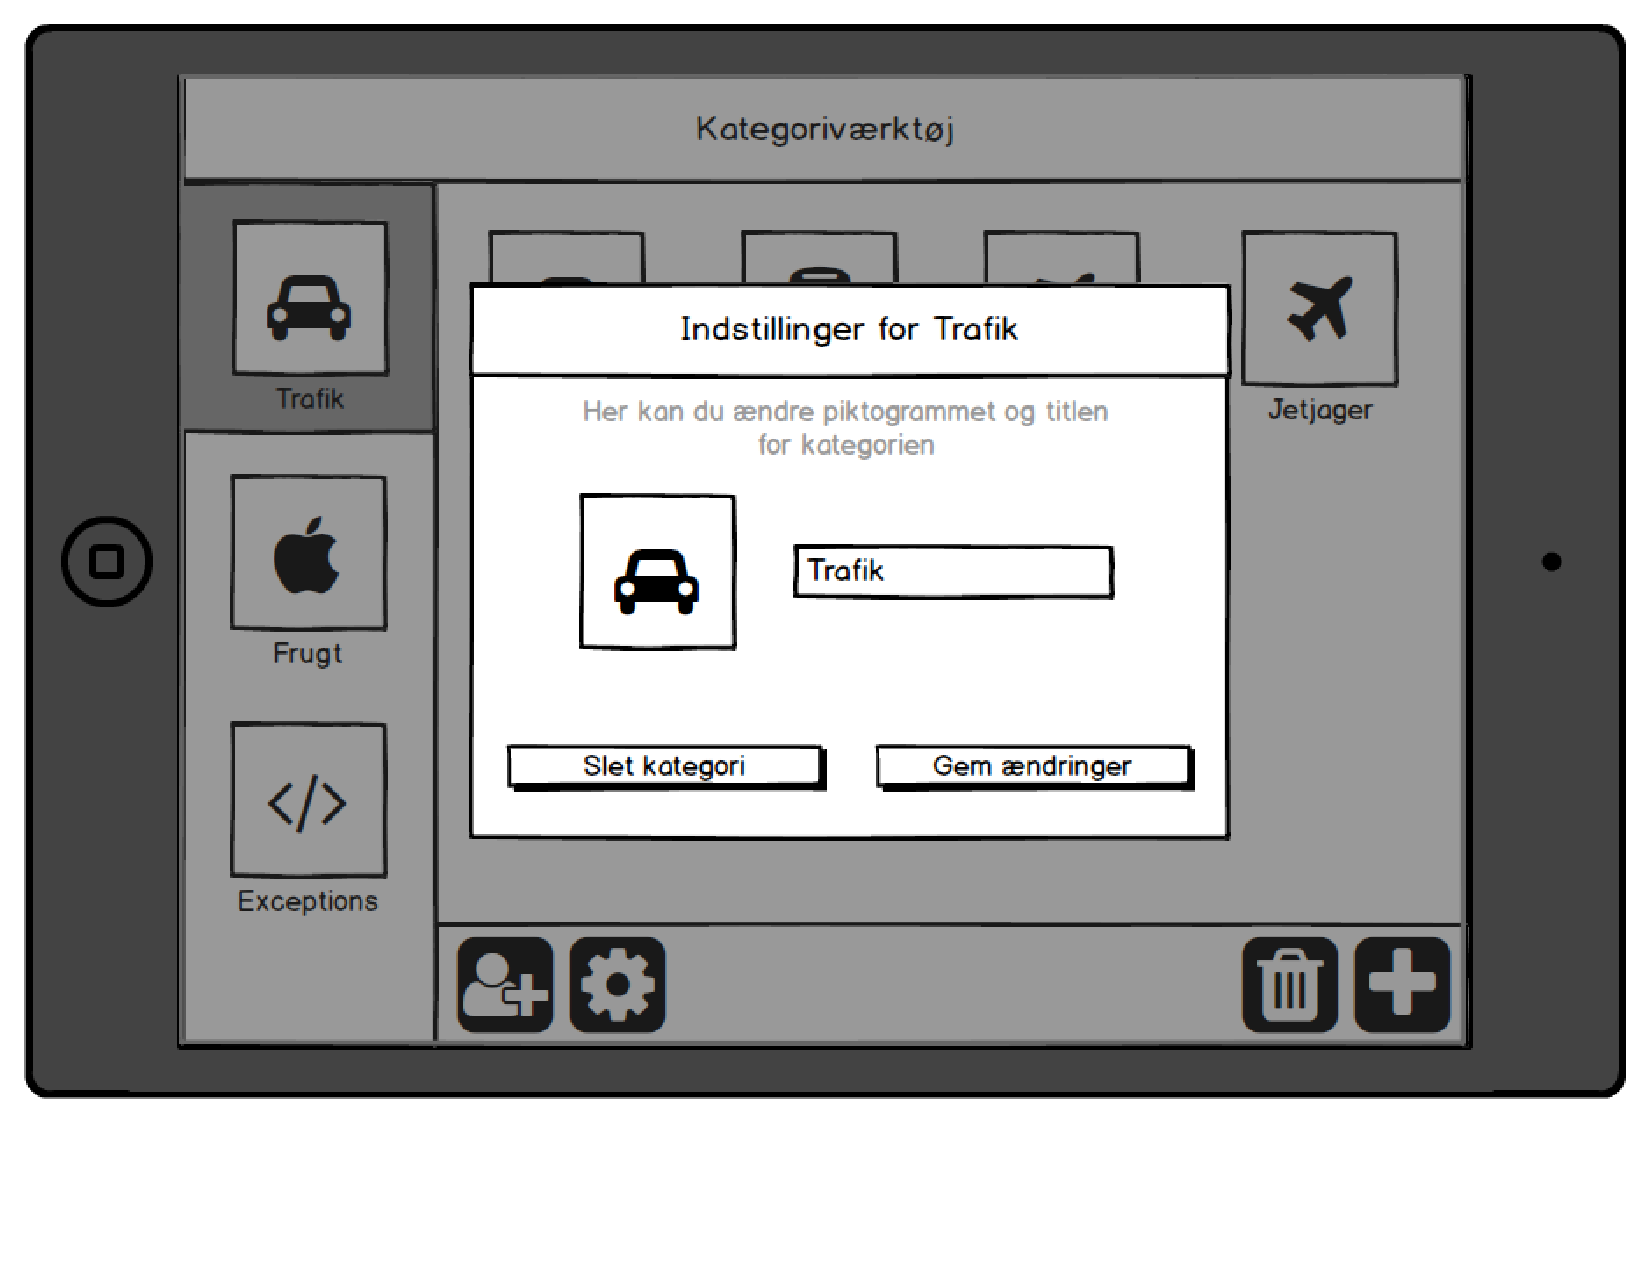
\includegraphics[width=0.75\textwidth]{sprint_two/improved_design/category_settings}
    \caption{Markup of the settings-dialog for a category}
    \label{fig:improved_design_category_settings}
\end{figure}

\FloatBarrier